\documentclass[xcolor=dvipsnames,aspectratio=1610]{beamer}

\usetheme{CambridgeUS}
\usefonttheme[onlylarge]{structurebold}
\setbeamerfont*{frametitle}{size=\normalsize,series=\bfseries}

\definecolor{myblue}{RGB}{5,5,200}
\definecolor{myorange}{RGB}{200,100,5}

\setbeamercolor*{structure}{bg=myblue!20,fg=myblue}

\setbeamercolor*{palette primary}{use=structure,fg=white,bg=structure.fg}
\setbeamercolor*{palette secondary}{use=structure,fg=white,bg=structure.fg!75}
\setbeamercolor*{palette tertiary}{use=structure,fg=white,bg=myorange}
\setbeamercolor*{palette quaternary}{fg=white,bg=myorange}

\setbeamercolor{section in toc}{fg=myorange,bg=white}
\setbeamercolor{alerted text}{use=structure,fg=structure.fg!50!black!80!black}

\setbeamercolor{titlelike}{parent=palette primary,fg=structure.fg!50!black}
\setbeamercolor{frametitle}{bg=myblue!85,fg=white}

\setbeamercolor*{titlelike}{parent=palette primary}

%\setbeamerfont{caption}{series=\normalfont,size=\fontsize{8}{8}} 

\setbeamertemplate{itemize item}[circle]
\setbeamertemplate{navigation symbols}{}
\setbeamertemplate{bibliography item}{}

\setbeamertemplate{footline}[frame number]

\newcommand\independent{\protect\mathpalette{\protect\independenT}{\perp}}
\def\independenT#1#2{\mathrel{\rlap{$#1#2$}\mkern2mu{#1#2}}}

\usepackage{amsmath}
   \usepackage{bm,amssymb, amsmath, graphicx}
   \usepackage{booktabs}
   \usepackage{caption}
\usepackage{subcaption}
\usepackage{float}
\usepackage{mathrsfs}
\usepackage{array} 
\usepackage{rotating}
\usepackage{amsthm}
\usepackage{eulervm}
\usepackage{mathtools}
\usepackage{boxedminipage}
\usepackage{tabularx}

\usepackage{fancyhdr}
\usepackage{hyperref}
\usepackage{graphicx}
\newcounter{qcounter}
\usepackage{caption}
\captionsetup{font=scriptsize,labelfont=scriptsize}
\usepackage{subcaption}
\usepackage[maxfloats=40]{morefloats}
\usepackage{float}

\usepackage{multirow}
\usepackage{rotating}
\usepackage{amsmath,amssymb}
\usepackage{appendixnumberbeamer}
\usepackage{algorithm,algpseudocode}
\usepackage{tkz-graph}
\usetikzlibrary{arrows,positioning,automata}
\usepackage{blkarray}% http://ctan.org/pkg/blkarray
\usepackage{comment}
\usepackage{natbib}
\usepackage{bibentry}

\newcommand{\matindex}[1]{\mbox{\scriptsize#1}}% Matrix index

\makeatletter
\renewcommand*\env@matrix[1][c]{\hskip -\arraycolsep
  \let\@ifnextchar\new@ifnextchar
  \array{*\c@MaxMatrixCols #1}}
\makeatother

\newcommand{\norm}[1]{\left|\left|#1\right|\right|}
\newcommand{\tr}{\mbox{tr}}
\newcommand{\RSS}{\mbox{RSS}}
\newcommand{\BIC}{\mbox{BIC}}
\newcommand{\Card}{\mbox{Card}}
\newcommand{\Tr}{\mbox{Tr}}
\newcommand{\abs}[1]{\left|#1\right|}
\newcommand{\E}{\mathbb{E}}
\newcommand{\var}[1]{\mbox{Var}\left(#1\right)}
\newcommand{\cov}[1]{\mbox{Cov}\left(#1\right)}
\newcommand{\cur}{\mbox{\scriptsize current}}
\newcommand{\old}{\mbox{\scriptsize old}}
\DeclareMathOperator*{\sign}{sign}
\DeclareMathOperator*{\cor}{cor}
\DeclareMathOperator*{\trace}{trace}
\DeclareMathOperator*{\argmax}{argmax}
\DeclareMathOperator*{\argmin}{argmin}
\newcommand{\spc}{\mbox{\scriptsize spc}}
\newcommand{\sym}{\mbox{\scriptsize sym}}
\newcommand{\con}{\mbox{\scriptsize con}}
\newcommand{\spl}{\mbox{\scriptsize spl}}
\newcommand{\uni}{\mbox{\scriptsize uni}}
\newcommand{\ones}{\mathbf 1}
\DeclareMathOperator{\est}{est}

\newcommand{\gored}{\color{Red}}
\newcommand{\goblk}{\color{Black}}
\newcommand{\gogrn}{\color{OliveGreen}}

\theoremstyle{remark} 
\newtheorem{rem}{Remark}


\title{Graphical Models}
\author{Syed Rahman\\\ \\
  \small Department of Statistics\\
  University of Florida}

\date{}

\begin{document}

{ % these braces make the change local to the single frame
  \setbeamertemplate{footline}{}
  \begin{frame}[noframenumbering]
  \vspace{1cm}
    \titlepage
  \end{frame}
}

%%%%%%%%%%%%%%%%%%%%%%%%%%%%%%%%%%%%%%%%%%%%%%%%%%
%% Introduction
%%%%%%%%%%%%%%%%%%%%%%%%%%%%%%%%%%%%%%%%%%%%%%%%%%

%\section{Introduction}

% { % these braces make the change local to the single frame
%   \setbeamertemplate{footline}{}
%   \begin{frame}[noframenumbering]
%     \begin{itemize}
%       \Large\centering\bf
%       \setlength{\itemsep}{20pt}
%     \item[] Why are graphical models useful?
%       selection
%     \end{itemize}
%   \end{frame}
% }

%\begin{frame}{Outline}
%  \begin{itemize}
%    \setlength{\itemsep}{26pt}
%  \item Introduction and motivation for graphical models 
%  \item Review of exisiting model selection approaches 
%  \item CONCORD: A new model selection approach 
%  \item Applications
%\end{itemize}
%\end{frame}

\begin{frame}{Motivation}
  \begin{itemize}
    \setlength{\itemsep}{10pt}
  \item Availability of high-dimensional data from various applications
  \item Number of variables ($p$) much larger than (or sometimes comparable to) the 
           sample size ($n$) 
  \item Examples:
    \begin{itemize}
      \setlength{\itemsep}{10pt}
    \item Biology: gene expression data
    \item Environmental science: climate data on spatial grid
    \item Finance: returns on thousands of stocks
    \end{itemize}
  \item Common goals: Understand complex relationships \& multivariate
      dependencies  
  \end{itemize}
\end{frame}

\begin{frame}{Modeling relationships}
  \begin{itemize}
    \setlength{\itemsep}{10pt}
    \item Covariance matrix $\Sigma$: a fundamental quantity to help understand 
     multivariate relationships
  %\item Estimates of $\Sigma$ required in procedures such as PCA, CCA,
    %MANOVA, etc.
  %\item Estimating $\Sigma$ is difficult in high dimensions
  \item Matrix $\Sigma$ of size $p$-by-$p$ has $O(p^2)$
    elements
  \item Estimating $O(p^2)$ parameters with classical estimators such as the 
  sample covariance matrix is not viable, especially when $n\ll p$ 
   \item {\bf Reliably estimate small number of parameters} in $\Sigma$ or $\Omega = \Sigma^{-1}$ 
  \item Set insignificant parameters to zero, giving rise to sparse estimates of $\Sigma$ or $\Omega$ 
 %\item Need novel methodology/tools to develop effective inferential
    %  procedures for analyzing high-dimensional data 
  \end{itemize}
\end{frame}

\begin{frame}{Concentration Graphical Models: Sparsity in $\Omega$}
  \begin{itemize}
    \setlength{\itemsep}{16pt}
  % \item Given iid observations $y_i^k$ with $k=1,\dots,n$ and
  %   $i=1,\dots,p$
  %   \begin{itemize}
  %   \item $n$: sample size, $p$: variables (nodes) 
  %   \item ${\bf Y}^{(k)}:=(y_1^k,\dots,y_p^k)$: $k$-th observation
  %   \item ${\bf Y}_i:=(y_i^1,\dots,y_i^n)'$: $i$-th variable
  %   \item ${\bf Y}^{(1)},\dots,{\bf Y}^{(k)}$: iid mean zero,
  %     covariance $\Sigma$ random variable
  %   \end{itemize}
  \item Let $Y$ be a $p$-dimensional random vector with a $N_p ( 0, \Sigma = 
  \Omega^{-1})$ distibution 
  %\item Denote $V=\{1,2,\dots,p\}$
  %\item Covariance matrix $cov(Y)=\Sigma$ encodes marginal
    %dependencies
    %$$ Y_i \independent Y_j \Longleftrightarrow 
    %cov(Y_i,Y_j) = [\Sigma]_{ij} = 0 $$
  \item $\Omega = ((\omega_{ij}))_{1 \leq i,j \leq p}$ 
  \item $\omega_{ij} = Cov(Y_i, Y_j \mid {Y}_{-(i,j)})$ 
  \item $\omega_{ij} = 0$ if and only if the $i^{th}$ and 
  $j^{th}$ variables are conditionally independent given the other variables 
  \item Zeros in $\Omega$ encode conditional independence under Gaussianity 
  %\item Also known as Markov Random Fields (MRF)
  \end{itemize}
\end{frame}

  \begin{frame}{Concentration Graphical Models: Connections with graphs}
  \begin{itemize}
    \setlength{\itemsep}{16pt}
\item The sparsity pattern in $\Omega$ can be represented by a graph, $G = (V,E)$. 
\item $V=\{1,\dots,p\}$ and set $E$ of edges is such that  $\omega_{ij} \neq 0 \Leftrightarrow (i,j) \in E$. 
  \end{itemize}
  \begin{table}
    \centering
    \begin{tabular}{MM}
      $ \Omega = \begin{blockarray}{c@{\hspace{5pt}}rrrr@{\hspace{5pt}}cl}
          & \matindex{A} & \matindex{B} & \matindex{C} &  \matindex{D} & &\\
          \begin{block}{(c@{\hspace{5pt}}rrrr@{\hspace{5pt}}c)l}
            &  4.29 & 0.65 & 0 & 0.8 && \matindex{A} \\
            & 0.65  & 4.25 & 0.76 & 0 && \matindex{B} \\
            & 0 & 0.76 & 4.16 & 0.8 && \matindex{C} \\
	& 0.80 & 0 & 0.80 & 4 && \matindex{D} 	\\
          \end{block}
        \end{blockarray}
        $ &
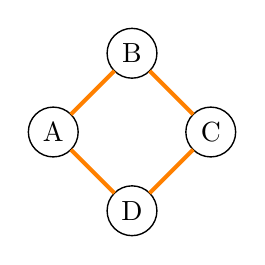
\begin{tikzpicture}
 \SetUpEdge[lw         = 1.5pt,
            color      = orange,
            labelcolor = white]
\tikzset{every node/.style={fill=white}} 
 \tikzset{VertexStyle/.append  style={fill}}
  \Vertex{A}
  \NOEA(A){B}  \SOEA(B){C} \SOEA(A){D}
\tikzset{EdgeStyle/.style={-}} 
\Edge[](A)(B)
  \Edge[](A)(D)
  \Edge[](B)(C)
\Edge[](C)(D)
\end{tikzpicture}
    \end{tabular}
  \end{table}
\end{frame}

\begin{frame}{Maximum Likelihood Estimation?}
  \begin{itemize}
    \setlength{\itemsep}{10pt}
  \item \Obtain a sparse estimate for $\Omega$ by maximizing
    the constrained objective function:
\begin{equation} \label{eq:glasso}
\hat{\Omega} = \argmax_{\Omega \succ 0} \underbrace{ - \trace (\Omega S) + log |\Omega|}_{\text{log-likelihood}} + \underbrace{\lambda \norm{\Omega}_1}_{\begin{subarray}{l}\text{penalty term to}\\
    \text{induce sparsity/zeros}\end{subarray}}
\end{equation}
\item Note that $\norm{\Omega}_1 = \max_{\norm{U}_{\infty} \leq 1} \trace (\Omega U) $
\item Thus we can rewrite the problem in Equation \ref{eq:glasso} as 
\begin{equation} \label{glasso2}
\max_{\Omega \succ 0} \min_{\norm{U}_{\infty} \leq 
\lambda} - \trace (\Omega(S + U)) + log |\Omega|
\end{equation}
  %\item $S$: sample covariance matrix
  %\item Graphical Lasso [Friedman, Hastie, \& Tibshirani, 2008]
  % \item Can we generalize GGM to a broader setting?
  %\item $\Omega$ can be computed by solving optimization problem
  \end{itemize}
\end{frame}

\begin{frame}{Dual Problem:}
  \begin{itemize}
    \setlength{\itemsep}{10pt}
  \item This is equivalent to solving:
\begin{equation} \label{dualglasso}
\min_{\norm{U}_{\infty} \leq \lambda}  \max_{\Omega \succ 0}- \trace (\Omega(S + U)) + log |\Omega|
\end{equation}
where
\begin{equation*} \label{indualglasso}
\argmax_{\Omega \succ 0}- \trace (\Omega(S + U)) + log |\Omega| = (S+U)^{-1}
\end{equation*}
by solving the basic maximum likelihood problem as $S+U \succ 0$.
\item Thus 
\begin{equation*} 
\max_{\Omega \succ 0}- \trace (\Omega(S + U)) + log |\Omega| = - p + \log|(S+U)^{-1}|
\end{equation*}
  \end{itemize}
\end{frame}

\begin{frame}{Dual Problem:}
  \begin{itemize}
    \setlength{\itemsep}{10pt}
\item Hence Equation \ref{dualglasso} becomes 
\begin{equation*} \label{dualglasso2}
&\min_{\norm{U}_{\infty} \leq \lambda}  - p - \log\abs{S+U} 
\end{equation*}
\item If we set $W = S + U$ we can instead focus on
\begin{equation*} \label{dualglasso2}
&\max_{\norm{W - S}_{\infty} \leq \lambda}  \log \abs{W}
\end{equation*}
where $\hat{\Sigma} = \max \{\log \abs{W} : {\norm{W - S}_{\infty} \leq \lambda} \}$
  \end{itemize}
\end{frame}

\begin{frame}{Dual Problem:}
  \begin{itemize}
    \setlength{\itemsep}{10pt}
\item Recall that $|W| = |W_{-j,-j}||W_{j,j}-W_{-j,j}^TW_{-j,-j}^{-1}W_{j,-j}|$. Assume $|W_{-j,-j}|$ is fixed and set $W_{kk} = S_{kk} + \lambda$ for all k.
\item Hence to maximize $\abs{W}$, we only need to minimize  $W_{-j,j}W_{-j-,j}^{-1}W_{j,-j}$ with respect to $W_{-j,j}$. This is equivalent to solving the following problem:
\begin{equation*} \label{optim}
\min_{w} w^T W_{j,j}^{-1} w \text{ subject to } \norm{w-S_j}_{\infty} \leq \lambda
\end{equation}
\item The dual of this problem is
\begin{equation} \label{optimdual}
\min_w w^T W_{-j,-j} w - S_j^Tw + \lambda \norm{w}_1
\end{equation}
as the dual norm of $\norm{.}_{\infty}$ is $\norm{.}_{1}$.
  \end{itemize}
\end{frame}

\begin{frame}{Connection to Lasso:}
  \begin{itemize}
    \setlength{\itemsep}{10pt}
\item Setting $Q = W_{-j,-j}^{\frac{1}{2}}$ and $b = \frac{1}{2}Q^{-1}S_j$ this problem becomes
\begin{equation*} \label{duallasso}
\min_w \norm{Qw-b}_2^2 + \lambda \norm{w}_1
\end{equation*}
which is a standard lasso problem.
\item We can also write this as
\begin{equation} \label{duallasso2}
\min_{\beta} \frac{1}{2} \norm{\Sigma_{11}^{1/2} \beta - b}_2^2 + \lambda \norm{\beta}_1
\end{equation}
where $b = \Sigma_{11}^{-1/2} s_{12}$
  \end{itemize}
\end{frame}

\begin{frame}{Graphical Lasso:}
  \begin{itemize}
    \setlength{\itemsep}{10pt}
\item One can also go directly from Equation \ref{eq:glasso} to \ref{optimdual}. Note that the subgradient equation for Equation \ref{eq:glasso} is
\begin{equation} \label{subgglasso}
\Omega^{-1} - S - \lambda \Gamma = 0 
\end{equation}
where $\Gamma_{ij} = \sign(\Omega_{ij}) \in [-1,1]$
\item Consider the partitons 
\begin{equation*}
\begin{pmatrix} 
\Sigma_{11}&\Sigma_{12}\\
\Sigma_{21}&\Sigma_{22}\\
\end{pmatrix} 
\begin{pmatrix} 
\Omega_{11}&\Omega_{12}\\
\Omega_{21}&\Omega_{22}\\
\end{pmatrix}
= \begin{pmatrix} 
I_{p-1,p-1}&0\\
0^T&1\\
\end{pmatrix}
\end{equation*}
  \end{itemize}
\end{frame}

\begin{frame}{Graphical Lasso:}
  \begin{itemize}
    \setlength{\itemsep}{10pt}
\item If we focus on the top right corner, we get 
\begin{equation} \label{subgglasso2}
\Sigma_{12} - s_{12} - \lambda \gamma_{12} = 0 
\end{equation}
\item The subgradient equations for Equation \ref{duallasso2} is
\begin{equation} \label{subgglasso3}
\Sigma_{11} \beta - s_{12} + \lambda \nu = 0 
\end{equation}
where $\nu_j = \sign(\beta_j) \in [-1,1]$
\item Now if $(\Sigma, \Gamma)$ solves Equation \ref{subgglasso}, then $(\Sigma_{12}, \gamma_{12})$ solves Equation \ref{subgglasso2}. In such a  case $\beta = \Sigma_{11}^{-1} \Sigma_{12}$ and $\nu = - \gamma_{12}$ solves Equation \ref{subgglasso3}. Hence equivalence of first 2 terms is obvious. 
  \end{itemize}
\end{frame}

\begin{frame}{Graphical Lasso:}
  \begin{itemize}
    \setlength{\itemsep}{10pt}
\item For the sign term, note that as $\Omega_{22}>0$,  we have that
\begin{align*}
 &\Sigma_{11} \Omega_{12} + \Sigma_{12} \Omega_{22} = 0 \\
\iff &\Omega_{12} = -\Omega_{22} \Sigma_{11}^{-1} \Sigma_{12} \\
\iff &\sign\{\Omega_{12}\} = \sign\{- \Sigma_{11}^{-1} \Sigma_{12}\} = -\sign{\beta}
\end{align*}
\item Finally note that solution of (\ref{duallasso2}) gives us a the corresponding part of $\Omega$: $&\Omega_{12} = -\Omega_{22} \beta$.
  \end{itemize}
\end{frame}

\begin{frame}{Neighborhood Selection:}
  \begin{itemize}
    \setlength{\itemsep}{10pt}
\item $ne_a \overset{def}{=} \{b \in V \setminus \{a\} \text{ s.t. } (a,b) \in E\} $
\item $cl_a \overset{def}{=} \{a\} \cup ne_a$
\item $\theta^a \overset{def}{=} \argmin_{\theta: \theta_a = 0} E(X_a - \sum_{b \in V} \theta_k X_k)^2$
\item For $b \in V \setminus \{a\}, \theta^a_b = -\Omega_{ab}/ \Omega_{aa}$ \implies $ne_a = \{b \in V: \theta^a_b \neq 0\}$
\item The lasso estimate $\hat{\theta^{a,\lambda}}$ of $\theta^a$ is
\begin{align*}
\hat{\theta^{a,\lambda}} = \argmin_{\theta: \theta_a = 0} (\frac{1}{n} \norm{X_a - X \theta}_2^2 + \lambda \norm{\theta}_1)
\end{align*}
where $ \norm{\theta}_1 = \sum_{b \in V} \abs{\theta_b}$
  \end{itemize}
\end{frame}

\begin{frame}{Neighborhood Selection:}
  \begin{itemize}
    \setlength{\itemsep}{10pt}
\item The neighborhood estimate (parametrized by $\lambda$)
\begin{align*}
\hat{ne}^{\lambda}_a = \{b \in V:  \hat{\theta_b^{a,\lambda}} \neq 0 \}
\end{align*}
\item Larger values of the penalty tend to shrink the size of the estimated set, while more variables are in general included into $\hat{ne}^{\lambda}_a$ if the value of $\lambda$ is diminished.
  \end{itemize}
\end{frame}

\begin{frame}{Large Sample Propoerties:}
  \begin{itemize}
    \setlength{\itemsep}{10pt}
\item Making some regularity assumptions we get some asymptotic consistency results: ($\hat{ne}^{\lambda}_a \not \subset ne_a \implies $ 0 in $\Omega$ and 1 in $\hat{\Omega}$)
\begin{align*}
P(\hat{ne}^{\lambda}_a \subset ne_a) = 1 - O(e^{-cn^{\epsilon}})
\end{align*}
for some $c>0$. This is Theorem 1 in the paper.
\item Theorem 2 state states ($ne_a  \not \subset \hat{ne}^{\lambda}_a \implies $ 1 in $\Omega$ and 0 in $\hat{\Omega}$)
\begin{align*}
P(ne_a \subset \hat{ne}^{\lambda}_a) = 1 - O(e^{-cn^{\epsilon}})
\end{align*}
for some $c>0$. 
\item Proofs begin from pg 23
  \end{itemize}
\end{frame}

\begin{frame}{Ising Model:}
  \begin{itemize}
    \setlength{\itemsep}{10pt}
\item Let $X_s \in \{-1,1\}$ for each vertex $s \in V$ and $\phi_{st}(x_s,x_t) = \theta^*_{st} x_s x_t$ for some parameter $\theta^*_{st} \in \mathbb{R}$, so that the distribution takes the form:
\begin{align*}
P_{\theta^*} (x) = \frac{1}{Z(\theta^*)} \exp \{ \sum_{(s,t) \in E} \theta^*_{st} x_s x_t \}
\end{align*}
where $Z(\theta^*)$ ensures that the distribution sums to 1.
\item For a graph $G = (V,E)$ over the $p$ variables, $\theta^*$ is a ${p \choose 2}$-dimensional vector where $\theta_{st} \neq 0 \iff (s,t) \in E$. In addition 
$$
X_s \perp X_t | X_{ V \backslash \{s,t\}} \iff \theta^*_{st} = 0 \text{ and } \theta^*_{ts} = 0
$$
\item The goal is to recover the \textit{signed edge set} $E^*$, where
\begin{align*}
E^* = \begin{cases}
\sign (\theta^*_{st}) & \text{ if } (s,t) \in E \\
0 & \text{ otherwise }
\end{cases}
\end{align*}
  \end{itemize}
\end{frame}

\begin{frame}{Neighborhood-based logistic regression:}
  \begin{itemize}
    \setlength{\itemsep}{10pt}
\item Recovering $E^*$ of an undirected graph is equivalent to recovering, for each vertex $r \in V$, its \textit{neighbothood set}, $\mathcal{N}(r) = \{t \in V | (r,t) \in E\}$ along with the correct $\sign(\theta^*_{rt}) \forall t \in \mathcal{N}(r)$. Define the \textit{signed neighborhood set} as 
\begin{align*}
\mathcal{N}_{\pm}(r) := \{\sign(\theta^*_{rt})t | t \in \mathcal{N}(r)\}
\end{align*}
\item $\theta^*_{\backslash r} := \{\theta^*_{ru}, u \in V \backslash r\}$
\item Note that the conditional distribution of $X_r$ given all the other variables, $X_{\backslash r}$ is 
\begin{align*}
P(x_r|x_{\backslash r}) = \frac{\exp(2x_r \sum_{t \in V \backslash r} \theta^*_{rt} x_t )}{\exp(2x_r \sum_{t \in V \backslash r } \theta^*_{rt} x_t ) + 1}
\end{align*}
which can be viewed as the logisitic regression of $X_r$ on $X_{\backslash r}$.
  \end{itemize}
\end{frame}

\begin{frame}{Neighborhood-based logistic regression:}
  \begin{itemize}
    \setlength{\itemsep}{10pt}
\item Given $n$ i.i.d samples $X = X^{(1)},...,X^{(n)}$, perform logistic regressionof each node $X_r$ on $X_{\backslash r}$ to estimate neighborhood structure $\hat{\mathcal{N}}_{\pm} (r).$ For each $r \in V$ solve the following problem
\begin{align} \label{eq:logis}
\min_{\theta_{\backslash r}} \{\ell(\theta;X) + \lambda_{(n,p,d)} \norm{\theta_{\backslash r}}_1\}
\end{align}
where 
\begin{align*}
\ell(\theta;X) := - \frac{1}{n} \sum_{i=1}^n \log P_\theta(x^{(i)}_r | x^{(i)}_{\backslash r})
\end{align*}
\item Then $\hat{\mathcal{N}}_{\pm}(r):= \{\sign(\hat{\theta}_{ru})u | u \in V \backslash r, \hat{\theta}_{ru} \neq 0 \}$ 
\item $\{\hat{E}_n = E^*\} \iff \forall r \in V, \hat{\mathcal{N}}_{\pm}(r) = {\mathcal{N}}_{\pm}(r)$
  \end{itemize}
\end{frame}

\begin{frame}{Large sample properties:}
  \begin{itemize}
    \setlength{\itemsep}{10pt}
\item Suppose $\lambda_n \geq \frac{16(2-\alpha)}{\alpha} \sqrt{\frac{\log p}{n}}$. Then there exists positive constants $L$ and $K$, independent of $(n,p,d)$ ($p$ is the number of nodes, $d$ is the maximum node degree) such that if $n > Ld^3 \log p$, then the following propoerties hold with probability at least $1-2\exp(-K\lambda_n^2n)$
\begin{enumerate}
\item For each node $r \in V$, the $\ell_1$ regularized logistic regression (\ref{eq:logis}), given the data $X$, has a unique solution, and so uniquely specifies a signed neighborhood $\hat{\mathcal{N}}_{\pm}(r)$
\item For each $r \in V$, the estimated signed neighborhood $\hat{\mathcal{N}}_{\pm}(r)$ correctly excludes all edges not in the true neighborhood. Moreoever, it correctly includes all edges $(r,t)$ for which $\abs{\theta_{rt}^*} \geq \frac{10}{C_{min}} \sqrt{d} \lambda_n$
\end{enumerate}
\item Hence the probability with which the method recovers the true signed edge-set decays exponentially fast as a function of $\lambda_n^2n$
  \end{itemize}
\end{frame}

\begin{frame}{Model Selection Consistency: Assumptions}
  \begin{itemize}
    \setlength{\itemsep}{10pt}
\item Consider a sequence of Ising models with graph edge sets $\{E^*_{p(n)}\}$ and parameters $\{\theta^*_{(n,p,d)}\}$; each of which satisfies the dependency (bounded eigenvalue) conditions and the incoherence conditions. 
\item For each $n$, let $X^n$ be an i.i.d sample specified by $\theta^*_{(n,p,d)}$ and suppose that $(n,p(n),d(n))$ satisfies $n > Ld^3 \log p$. 
\item Suppose further that $\lambda_n \geq \frac{16(2-\alpha)}{\alpha} \sqrt{\frac{\log p}{n}}$ and $\lambda_n^2 n \to 0$ and the minimum parameter weights satisfy 
$$
\min_{(r,t) \in E^*_n} \abs{\theta^*_{(n,p,d)}(r,t)} \geq \frac{10}{C_{min}} \sqrt{d} \lambda_n
$$ 
for sufficiently large $n$. 
  \end{itemize}
\end{frame}

\begin{frame}{Model Selection Consistency: Result}
  \setbeamercolor{eecks} {bg=Orange, fg=Blue}
\vspace{.5in}
  \begin{beamercolorbox}[shadow=true, rounded=true]{eecks}
\centering {Then the method is model selection consistent so that if $\hat{E}_{p(n)}$ is the graph structure estimated by the data $X^n$, then $P[\hat{E}_{p(n)} = {E}^*_{p(n)}] \to 1$ as $n \to \infty$.}
 \end{beamercolorbox}
\end{frame}

\begin{frame}{Motivation for Joint Estimation}
  \begin{itemize}
    \setlength{\itemsep}{10pt}
\item As mentioned before, graphical models are of particular interest in the analysis of gene expression data since they can provide a useful tool for visualizing the relationships among genes and generating biological hypotheses. 

\item The datasets may correspond to several distinct classes. For example, suppose a cancer researcher collects gene expression measurements for a set of cancer tissue samples and a set of normal tissue samples.  One might want to estimate a graphical model for the cancer samples and a graphical model for the normal samples.

\item One might expect the two graphical models to be similar to each other since both are based on the same type of tissue, but also have important differences resulting from the fact that gene networks are often dysregulated in cancer. 
  \end{itemize}
\end{frame}

\begin{frame}{Problem Formulation}
  \begin{itemize}
    \setlength{\itemsep}{10pt}
  \item Suppose we have a heterogeneous data set with $p$ variables and $K$ categories.
  
   \item The $k$-th
  category contains $n_k$ observations $(\boldsymbol{x}_1^{(k)},...,\boldsymbol{x}_{n_k}^{(k)})$, where each $\boldsymbol{x}_i^{(k)} = (x_{i,1}^{(k)},...,x_{i,p}^{(k)})$ is a $p$-dimensional row vector.

   \item Without loss of generality, we assume the observations in the same category are centered along each variable, i.e., $\sum_{i=1}^{n_k} x_{i,j}^{(k)} = 0$ for all $1 \leq j \leq p$ and $1 \leq k \leq K$.

\item So we solve the basic prpblem: 
\begin{equation*}
     \underset{\Omega^{(k)}}{\mbox{min}} \  \mbox{trace} (\hat{\Sigma}^{(k)} \Omega^{(k)}) - \log\{ \det(\Omega^{(k)})\} + \lambda_k \sum_{j \neq j'} |\omega_{j,j'}^{(k)}|,
\end{equation*}
by reparameterizing $\omega_{j,j'}^{(k)}$  as     
      \begin{equation*}
     \omega_{j,j'}^{(k)} = \theta_{j,j'} \gamma_{j,j'}^{(k)}, 1\leq j \neq j' \leq p, \ 1\leq k \leq K 
\end{equation*}
  \end{itemize}
\end{frame}

\begin{frame}{Joint Estimation}
  \begin{itemize}
    \setlength{\itemsep}{10pt}
\item          Let $\Theta = (\theta_{j,j'})_{p\times p}$ and $\Gamma^{(k)} = (\gamma_{j,j'}^{(k)})_{p\times p}$. To estimate this model, the following penalized criterion is used:
        
        \
        \begin{equation}
        \underset{\Theta,\{ \Gamma^{(k)}\}_{k=1}^{K}}{\min}   \sum_{k=1}^{K} [\mbox{trace}(\hat{\Sigma} \Omega^{(k)}) - \log\{ \det(\Omega^{(k)})\}] \ +  \eta_1 \underset{j \neq j'}{\sum} \theta_{j,j'} +   
        \eta_2 \underset{j \neq j'}{\sum} \sum_{k=1}^K |\gamma_{j,j'}^{(k)}|,
        \end{equation}
        \
        
        subject to    $ \ \ \omega_{j,j'}^{(k)}=\theta_{j,j'} \gamma_{j,j'}^{(k)}$, $\theta_{j,j'} > 0$, $1 \leq j,j' \leq p$
        
        $\ \ \ \ \ \ \ \ \ \ \ \ \ \ \ \ \theta_{j,j'} = \theta_{j',j}$, $\gamma_{j,j'}^{(k)} = \gamma_{j',j}^{(k)}, 1 \leq j \neq j' \leq p$; $1 \leq k \leq K$
        
        $\ \ \ \ \ \ \ \ \ \ \ \ \  \ \ \ \theta_{j,j'}=1,\gamma_{j,j}^{(k)}=\omega_{j,j'}^{(k)} , 1 \leq j = j' \leq p$; $1 \leq k \leq K$,
        
        \
        
        where $\eta_1$ and $\eta_2$ are two tuning parameters. 

  \end{itemize}
\end{frame}


\begin{frame}{Joint Estimation}
  \begin{itemize}
    \setlength{\itemsep}{10pt}
\item   
Suppose we have data from $K \geq 2$ distinct classes.  Instead of estimating $\bm{\Sigma}_{1}^{-1},\bm{\Sigma}_{2}^{-1},\ldots,\bm{\Sigma}_{K}^{-1}$ separately, we estimate these values jointly by maximizing the following penalized log-likelihood function
\small
\begin{equation*}
\max_{\{\bm{\Theta}\}} \sum_{k=1}^{K}n_{k}\left[\log\,\det \bm{\Theta}^{(k)}-\mbox{trace}\left(\bm{S}^{(k)}\bm{\Theta}^{(k)}\right)\right] - P(\{\bm{\Theta}\}),
\end{equation*}
\normalsize
subject to the constraint that $\bm{\Theta}^{(1)},\bm{\Theta}^{(2)},\ldots,\bm{\Theta}^{(K)}$ are positive definite, where $\{\bm{\Theta}\} = \{\bm{\Theta}^{(1)},\bm{\Theta}^{(2)},\ldots,\bm{\Theta}^{(K)}\}$.

\item $P(\{\bm{\Theta}\})$ denotes a convex penalty function, so the objective function is strictly concave.
  \end{itemize}
\end{frame}

\begin{frame}{Joint Estimation}
  \begin{itemize}
    \setlength{\itemsep}{10pt}

\item The fused graphical lasso (FGL) penalty is given by
\small
\begin{equation*}
P(\{\bm{\Theta}\}) = \lambda_{1}\sum_{k=1}^{K}\sum_{i\neq j}|\theta_{ij}^{(k)}| + \lambda_{2}\sum_{k<k'}\sum_{i,j}|\theta_{ij}^{(k)}-\theta_{ij}^{(k')}|,
\end{equation*}
\normalsize
where $\lambda_{1}$ and $\lambda_{2}$ are nonnegative tuning parameters

\item The group graphical lasso (GGL) penalty function is given by
\small
\begin{equation*}
P(\{\bm{\Theta}\}) = \lambda_{1}\sum_{k=1}^{K}\sum_{i\neq j}|\theta_{ij}^{(k)}| + \lambda_{2}\sum_{i\neq j}\sqrt{\sum_{k=1}^{K}\theta_{ij}^{(k)^{2}}},
\end{equation*}
\normalsize
where $\lambda_{1}$ and $\lambda_{2}$ are nonnegative tuning parameters    
 
 \end{itemize}
\end{frame}

\begin{frame}
\frametitle{References}
\small
\begin{block}{}
\begin{thebibliography}{Tototo}
\bibitem{Banerjee} Banerjee, O. , El Ghaoui, L. and  d’Aspremont, A.  (2008), {``Model Selection Through Sparse Maximum Likelihood Estimation
for Multivariate Gaussian or Binary Data,''} \emph{Journal of Machine Learning Research}, 9  485-516
\bibitem{Meinshausen}  Meinshausen, N. and Buhlmann, P. (2006), {``High-dimensional Variable Selectiuon Using the Lasso,''} \emph{The Annals of Statistics}, Vol. 34, No. 3, 1436–1462
\bibitem{Ravimukar}  Ravikumar, P, Wainwright, M. J., Lafferty, J. D. (2010), {``High-dimensional Ising model selection using $\ell-1$-regularized logistic regression,''} \emph{The Annals of Statistics}, 38 (2010), no. 3, 1287--1319. doi:10.1214/09-AOS691
\bibitem{Danaher} Danaher, P., Wang, P., and Witten, D. (2014), {``The joint graphical lasso for inverse covariance estimation across multiple classes,''} \emph{Journal of the Royal Statistical Society: Series B (Statistical Methodology)}, 76(2), 373-397.
\bibitem{Guo} Guo, J., Levina, E., Michailidis, G., and Zhu, J. (2011), {``Joint Estimation of Multiple Graphical Models,''} \emph{Biometrika}, 98(1), 1-15. 
\end{thebibliography}
\end{block}
\end{frame}

\end{document}
